%%%%%%%%%%%%%%%%%%%%%%%%%%%%%%%%%%%%%%%%%
% Arsclassica Article
% LaTeX Template
% Version 1.1 (1/8/17)
%
% This template has been downloaded from:
% http://www.LaTeXTemplates.com
%
% Original author:
% Lorenzo Pantieri (http://www.lorenzopantieri.net) with extensive modifications by:
% Vel (vel@latextemplates.com)
%
% License:
% CC BY-NC-SA 3.0 (http://creativecommons.org/licenses/by-nc-sa/3.0/)
%
%%%%%%%%%%%%%%%%%%%%%%%%%%%%%%%%%%%%%%%%%

%----------------------------------------------------------------------------------------
%	PACKAGES AND OTHER DOCUMENT CONFIGURATIONS
%----------------------------------------------------------------------------------------

\documentclass[
12pt, % Main document font size
a4paper, % Paper type, use 'letterpaper' for US Letter paper
oneside, % One page layout (no page indentation)
%twoside, % Two page layout (page indentation for binding and different headers)
headinclude,footinclude, % Extra spacing for the header and footer
BCOR5mm, % Binding correction
]{scrartcl}
%%%%%%%%%%%%%%%%%%%%%%%%%%%%%%%%%%%%%%%%%
% Arsclassica Article
% Structure Specification File
%
% This file has been downloaded from:
% http://www.LaTeXTemplates.com
%
% Original author:
% Lorenzo Pantieri (http://www.lorenzopantieri.net) with extensive modifications by:
% Vel (vel@latextemplates.com)
%
% License:
% CC BY-NC-SA 3.0 (http://creativecommons.org/licenses/by-nc-sa/3.0/)
%
%%%%%%%%%%%%%%%%%%%%%%%%%%%%%%%%%%%%%%%%%

%----------------------------------------------------------------------------------------
%	REQUIRED PACKAGES
%----------------------------------------------------------------------------------------

\usepackage[
nochapters, % Turn off chapters since this is an article
beramono, % Use the Bera Mono font for monospaced text (\texttt)
eulermath,% Use the Euler font for mathematics  eulermath
pdfspacing, % Makes use of pdftex’ letter spacing capabilities via the microtype package
dottedtoc % Dotted lines leading to the page numbers in the table of contents
]{classicthesis} % The layout is based on the Classic Thesis style

\usepackage{arsclassica} % Modifies the Classic Thesis package

\usepackage[T1]{fontenc} % Use 8-bit encoding that has 256 glyphs

\usepackage[utf8]{inputenc} % Required for including letters with accents

\usepackage{graphicx} % Required for including images
\graphicspath{{Figures/}} % Set the default folder for images

\usepackage{enumitem} % Required for manipulating the whitespace between and within lists

\usepackage{lipsum} % Used for inserting dummy 'Lorem ipsum' text into the template

\usepackage{subfig} % Required for creating figures with multiple parts (subfigures)

\usepackage{amsmath,amssymb,amsthm} % For including math equations, theorems, symbols, etc

\usepackage{varioref} % More descriptive referencing

%----------------------------------------------------------------------------------------
%	THEOREM STYLES
%---------------------------------------------------------------------------------------

\theoremstyle{definition} % Define theorem styles here based on the definition style (used for definitions and examples)
\newtheorem{definition}{Definition}

\theoremstyle{plain} % Define theorem styles here based on the plain style (used for theorems, lemmas, propositions)
\newtheorem{theorem}{Theorem}

\theoremstyle{remark} % Define theorem styles here based on the remark style (used for remarks and notes)

%----------------------------------------------------------------------------------------
%	HYPERLINKS
%---------------------------------------------------------------------------------------

\hypersetup{
%draft, % Uncomment to remove all links (useful for printing in black and white)
colorlinks=true, breaklinks=true, bookmarks=true,bookmarksnumbered,
urlcolor=webbrown, linkcolor=RoyalBlue, citecolor=webgreen, % Link colors
pdftitle={}, % PDF title
pdfauthor={\textcopyright}, % PDF Author
pdfsubject={}, % PDF Subject
pdfkeywords={}, % PDF Keywords
pdfcreator={pdfLaTeX}, % PDF Creator
pdfproducer={LaTeX with hyperref and ClassicThesis} % PDF producer
}  % Include the structure.tex file which specified the document structure and layout
% Specify custom hyphenation points in words with dashes where you would like hyphenation to occur, or alternatively, don't put any dashes in a word to stop hyphenation altogether

%----------------------------------------------------------------------------------------
%	TITLE AND AUTHOR(S)
%----------------------------------------------------------------------------------------

\title{{Spatial Multilevel Fused Lasso model for large datasets}} % The article title \normalfont\spacedallcaps

%\subtitle{Subtitle} % Uncomment to display a subtitle
\author{{Yewen Chen}} %\spacedlowsmallcaps The article author(s) - author affiliations need to be specified in the AUTHOR AFFILIATIONS block

\date{\normalsize{October 13, 2020}}
 % An optional date to appear under the author(s)

%----------------------------------------------------------------------------------------
\usepackage[margin=0.8in]{geometry}
\usepackage{tgbonum}
\usepackage{amsmath}
\usepackage{natbib}
\usepackage{float}
\usepackage{algorithm}
\usepackage{algpseudocode}
\usepackage{color}
\usepackage{fancyvrb}
\usepackage{relsize}
\usepackage{hyperref}
\usepackage{url}
\usepackage{bbm}
\usepackage{threeparttable}
\usepackage{multirow}
\usepackage{longtable}
\usepackage{multicol}
\usepackage{makecell}


\hypersetup{
    colorlinks=true,
    linkcolor=blue,
    filecolor=magenta,
    urlcolor=cyan,
}
\makeatletter
\def\hlinewd#1{%
\noalign{\ifnum0=`}\fi\hrule \@height #1 %
\futurelet\reserved@a\@xhline}
\makeatother

\urlstyle{same}
\newcommand{\VerbBar}{|}
\newcommand{\VERB}{\Verb[commandchars=\\\{\}]}
\DefineVerbatimEnvironment{Highlighting}{Verbatim}{commandchars=\\\{\}}
% Add ',fontsize=\small' for more characters per line
\usepackage{framed}
\definecolor{shadecolor}{RGB}{248,248,248}
\newenvironment{Shaded}{\begin{snugshade}}{\end{snugshade}}
\newcommand{\AlertTok}[1]{\textcolor[rgb]{0.94,0.16,0.16}{#1}}
\newcommand{\AnnotationTok}[1]{\textcolor[rgb]{0.56,0.35,0.01}{\textbf{\textit{#1}}}}
\newcommand{\AttributeTok}[1]{\textcolor[rgb]{0.77,0.63,0.00}{#1}}
\newcommand{\BaseNTok}[1]{\textcolor[rgb]{0.00,0.00,0.81}{#1}}
\newcommand{\BuiltInTok}[1]{#1}
\newcommand{\CharTok}[1]{\textcolor[rgb]{0.31,0.60,0.02}{#1}}
\newcommand{\CommentTok}[1]{\textcolor[rgb]{0.56,0.35,0.01}{\textit{#1}}}

\newcommand{\DataTypeTok}[1]{\textcolor[rgb]{0.13,0.29,0.53}{#1}}
\newcommand{\DecValTok}[1]{\textcolor[rgb]{0.00,0.00,0.81}{#1}}
\newcommand{\DocumentationTok}[1]{\textcolor[rgb]{0.56,0.35,0.01}{\textbf{\textit{#1}}}}
\newcommand{\ErrorTok}[1]{\textcolor[rgb]{0.64,0.00,0.00}{\textbf{#1}}}

\newcommand{\FunctionTok}[1]{\textcolor[rgb]{0.00,0.00,0.00}{#1}}
\newcommand{\ImportTok}[1]{#1}
\newcommand{\InformationTok}[1]{\textcolor[rgb]{0.56,0.35,0.01}{\textbf{\textit{#1}}}}
\newcommand{\KeywordTok}[1]{\textcolor[rgb]{0.13,0.29,0.53}{\textbf{#1}}}
\newcommand{\NormalTok}[1]{#1}
\newcommand{\OperatorTok}[1]{\textcolor[rgb]{0.81,0.36,0.00}{\textbf{#1}}}
\newcommand{\OtherTok}[1]{\textcolor[rgb]{0.56,0.35,0.01}{#1}}
\newcommand{\PreprocessorTok}[1]{\textcolor[rgb]{0.56,0.35,0.01}{\textit{#1}}}
\newcommand{\RegionMarkerTok}[1]{#1}
\newcommand{\SpecialCharTok}[1]{\textcolor[rgb]{0.00,0.00,0.00}{#1}}
\newcommand{\SpecialStringTok}[1]{\textcolor[rgb]{0.31,0.60,0.02}{#1}}
\newcommand{\StringTok}[1]{\textcolor[rgb]{0.31,0.60,0.02}{#1}}
\newcommand{\VariableTok}[1]{\textcolor[rgb]{0.00,0.00,0.00}{#1}}
\newcommand{\VerbatimStringTok}[1]{\textcolor[rgb]{0.31,0.60,0.02}{#1}}
\newcommand{\WarningTok}[1]{\textcolor[rgb]{0.56,0.35,0.01}{\textbf{\textit{#1}}}}

\begin{document}
\renewcommand{\UrlFont}{\small\tt}
\bibliographystyle{abbrvnat}
\setlength{\abovecaptionskip}{0pt}
\setlength{\belowcaptionskip}{10pt}
%----------------------------------------------------------------------------------------
%	HEADERS
%----------------------------------------------------------------------------------------
\renewcommand{\algorithmicrequire}{\textbf{Input:}}  % Use Input in the format of Algorithm
\renewcommand{\algorithmicensure}{\textbf{Update step:}} % Use Output in the format of Algorithm
\renewcommand{\sectionmark}[1]{\markright{\spacedlowsmallcaps{#1}}} % The header for all pages (oneside) or for even pages (twoside)
%\renewcommand{\subsectionmark}[1]{\markright{\thesubsection~#1}} % Uncomment when using the twoside option - this modifies the header on odd pages
\lehead{\mbox{\llap{\small\thepage\kern1em\color{halfgray} \vline}\color{halfgray}\hspace{0.5em}\rightmark\hfil}} % The header style

\pagestyle{scrheadings} % Enable the headers specified in this block

%----------------------------------------------------------------------------------------
%	TABLE OF CONTENTS & LISTS OF FIGURES AND TABLES
%----------------------------------------------------------------------------------------

\maketitle % Print the title/author/date block

\setcounter{tocdepth}{4} % Set the depth of the table of contents to show sections and subsections only

\tableofcontents % Print the table of contents

\listoffigures % Print the list of figures

\listoftables % Print the list of tables

%----------------------------------------------------------------------------------------
%	ABSTRACT
%----------------------------------------------------------------------------------------
\newpage
%\section{\href{https://chenyw68.github.io/Literature[2020]spNNGP R package for Nearest Neighbor Gaussian Process models.pdf}{The nearest neighbor Gaussian process}}
%Similar to the pre-defined knots for Gaussian predictive processes, the starting point of nearest neighbor Gaussian process (NNGP) approach is to choose a fixed collection (e.g.,  $\boldsymbol{S}$) of distinct locations in $\boldsymbol{D}$, where $\boldsymbol{S}$ need not coincide with or be apart of the
%observed locations, so its size $k$ need not equal the size of the dataset $n$ (or \textcolor[rgb]{0.50,0.50,0.50}{even larger than the size $n$}). The set $\boldsymbol{S}$ is called as reference set by
%\href{https://chenyw68.github.io/Literature/[2016]Hierarchical nearest-neighbor Gaussian process models for large geostatistical datasets.pdf}{\cite{datta2016hierarchical}}.
%
%A directed acyclic graph is defined on the reference set $\boldsymbol{S}$, and then the joint distribution of spatial process $w(s)$ from the reference set is represented by the product of conditional densities which is motivated by Vecchia’s approximation \citep{vecchia1988estimation} ideas, where a careful choice of suitable conditional sets is required, and this conditional set is constrained to be the $m$-nearest neighbors by the NNGP approach, thereby facilitating computation in estimation and prediction problem (for more details on those problems, see  \href{https://chenyw68.github.io/Literature/[2016]Hierarchical nearest-neighbor Gaussian process models for large geostatistical datasets-Appdix.pdf}{Appendix} of \href{https://chenyw68.github.io/Literature/[2016]Hierarchical nearest-neighbor Gaussian process models for large geostatistical datasets.pdf}{\cite{datta2016hierarchical}} and \href{https://chenyw68.github.io/Literature/[2017]Applying Nearest Neighbor Gaussian Processes to Massive Spatial Data Sets.pdf}{\citep{finley2017applying}} and \href{https://chenyw68.github.io/Literature/[2019]Efficient algorithms for bayesian nearest neighbor gaussian processes.pdf}{\cite{finley2019efficient}}); \href{https://chenyw68.github.io/Literature/[2019]Distributed Implementation of Nearest-Neighbor Gaussian process.pdf}{the distributed Implementation}.
%
%Based on these results above, a NNGP can be well-defined from a parent Gaussian process $GP(\boldsymbol{0}, \boldsymbol{C\left(\cdot; \boldsymbol{\theta}\right)})$.
%
%%is defined from the conditional specification of the joint distribution of spatial process $w(s)$ in (\ref{model}), i.e. the joint distribution is
%%represented by the product of conditional densities which is motivated by \citet{vecchia1988estimation} ideas, where a careful choice of suitable conditional sets is required.
%
%%\textcolor[rgb]{1.00,0.00,1.00}{Comment:}
%\begin{itemize}
% \item [1)] Total operations is $O((n + k)m^3)$ where $m (\approx 20)$ is the size of conditioning set or neighbor set, and several processes can run in parallel (e.g, computations of weights in Kriging equation (\ref{Kriging})).
% \item [2)] The other major advantage is that the precision matrix of the NNGP is sparse with at most $km(m + 1)/2$ nonzero entries.
% \item [3)] NNGP can also be extended to large spatio-temporal data (
%\href{https://chenyw68.github.io/Literature/[2016]Nonseparable dynamic NNGP models for large spatio-temporal data.pdf}{\cite{datta2016nonseparable}}) and non-stationary process(\href{https://chenyw68.github.io/Literature/[2020]Computationally efficient nonstationary NNGP models using data-driven techniques.pdf}{\cite{konomi2019computationally}}), \href{https://chenyw68.github.io/Literature/[2020-formal]Bayesian inference for high dimensional nonstationary Gaussian processes.pdf}{\citep{risser2020bayesian}}.
%\end{itemize}
%
%
%\section{Two exploratory limitations of the NNGP approach}
%\subsection{Exploratory analysis }
%\begin{itemize}
% \item [1)]Problem 1: Since the joint distribution of spatial process $w(s)$ from the reference set is represented by using the product of conditional densities and those conditional sets are constrained to be the $m$-nearest neighbors, so $m$-nearest neighbors may fail to capture all the information about the covariance parameters when there is a true \textbf{large scale dependence} in the dataset.
% \item [2)]Problem 2: From an application point of view, the reference set $\boldsymbol{S}$ cannot be infinite because we need to solve neighbor set for every location, so the performance of the NNGP approximation depends on the size of the spatial dependence range relative to the spacing of the reference set, that maybe lead to the quality of the NNGP approximation gets worse when \textbf{the spatial dependence range gets shorter}.
%\end{itemize}

%With regard to Problem 1, some simulation results were given by \href{https://chenyw68.github.io/Literature/[2016]Hierarchical nearest-neighbor Gaussian process models for large geostatistical datasets.pdf}{\cite{datta2016hierarchical}} where they generated datasets of size 2500 in a unit square domain and considered estimation cases of different range parameters. Those results can be found in Figure \ref{fig:datta}.  Figure \ref{fig:datta} suggests that the NNGP model deliver inference similar to that of a full GP even for slow decaying covariance functions. However, Figure \ref{fig:datta} shows also that the NNGP obviously tends to underestimate the estimate of range parameter $\phi$ with the increase of spatial range $\phi$.
%\begin{figure}[H]
%{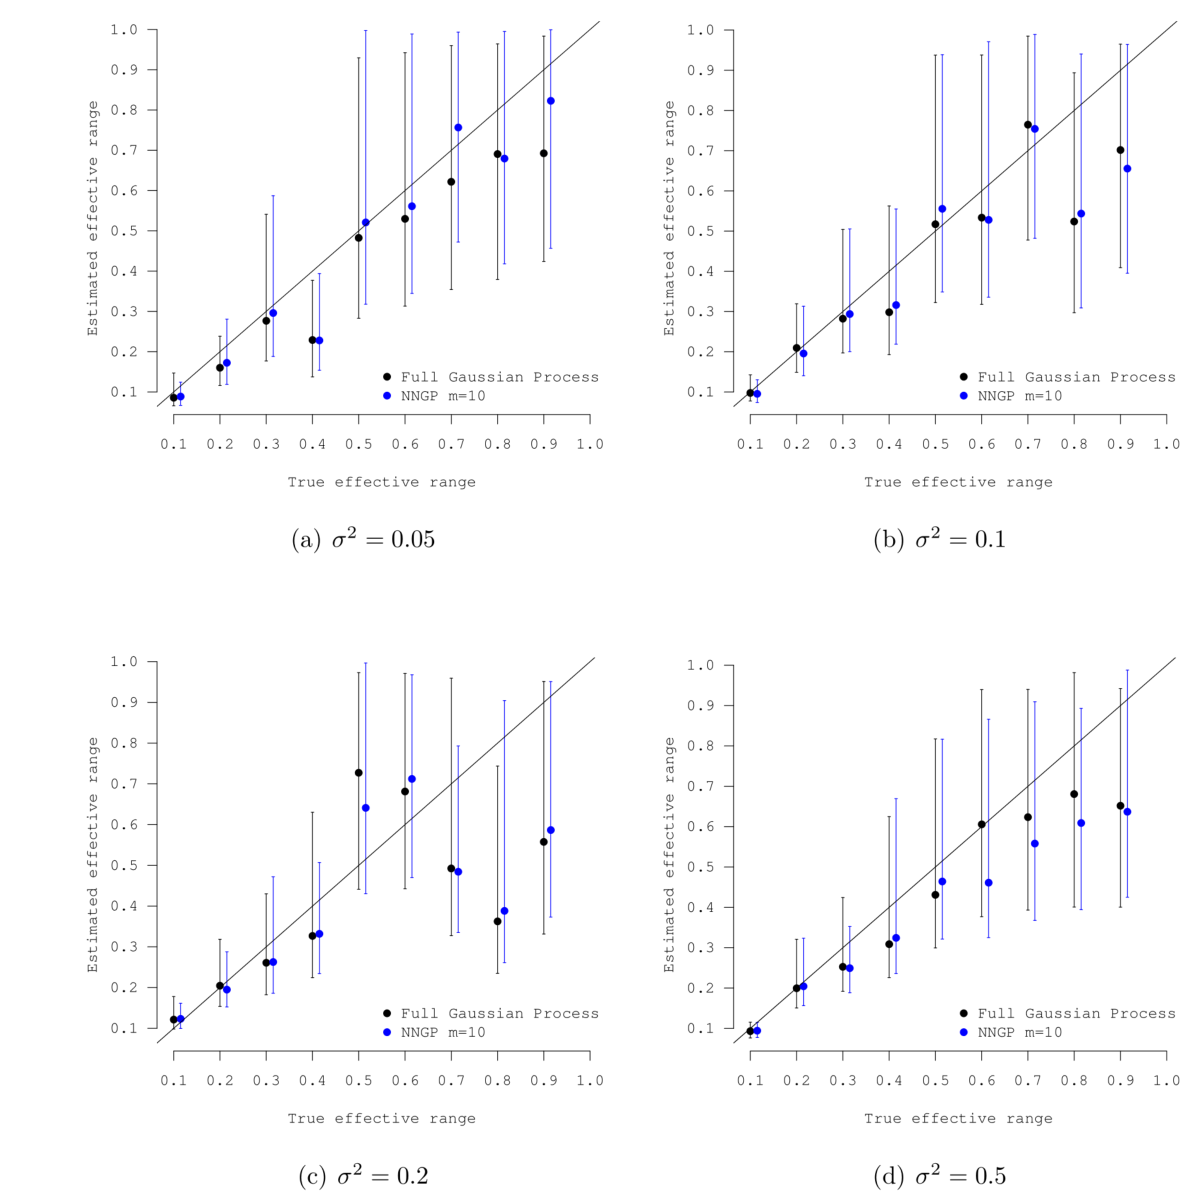
\includegraphics[width=16cm]{Figures/datta_NNGP.png} }
%\vspace{1em}
%\caption{Simulation results of \href{https://chenyw68.github.io/Literature/[2016]Hierarchical nearest-neighbor Gaussian process models for large geostatistical datasets.pdf}{\cite{datta2016hierarchical}}.}\label{fig:datta}
%\end{figure}


%We considered model (\ref{model}) with $\boldsymbol{\beta X} = 0.1\boldsymbol{I}, \sigma^2 = 5, \tau^2 = 1$, and the Matern correlation function for the spatial random effects $\boldsymbol{w}$, with a constant smoothness parameter $\nu = 0.5$ and varying spatial range parameters.
%
%Three distance criteria:
%\begin{align}
%D_{\mathrm{KL}}(\hat{\mathbf{\Sigma}}, \mathbf{\Sigma}) &=\frac{1}{2}\left[\operatorname{trace}\left(\hat{\mathbf{\Sigma}}^{-1} \mathbf{\Sigma}\right)- p +\log |\hat{\mathbf{\Sigma}}|-\log |\mathbf{\Sigma}|\right] \\
%D_{\mathrm{B}}(\hat{\mathbf{\Sigma}}, \mathbf{\Sigma}) &=\frac{1}{2} \log |\tilde{\mathbf{\Sigma}}|-\frac{1}{4}\log | \hat{\mathbf{\Sigma}} |-\frac{1}{4} \log | \mathbf{\Sigma} |, \quad \tilde{\mathbf{\Sigma}}=[\mathbf{\Sigma}+\hat{\mathbf{\Sigma}}] / 2 \\
%D_{\mathrm{F}}(\hat{\mathbf{\Sigma}}, \mathbf{\Sigma}) &=\sqrt{\operatorname{trace}\left[(\hat{\mathbf{\Sigma}}-\mathbf{\Sigma})(\hat{\mathbf{\Sigma}}-\mathbf{\Sigma})^{\prime}\right]}
%\end{align}

%\begin{figure}[H]
%{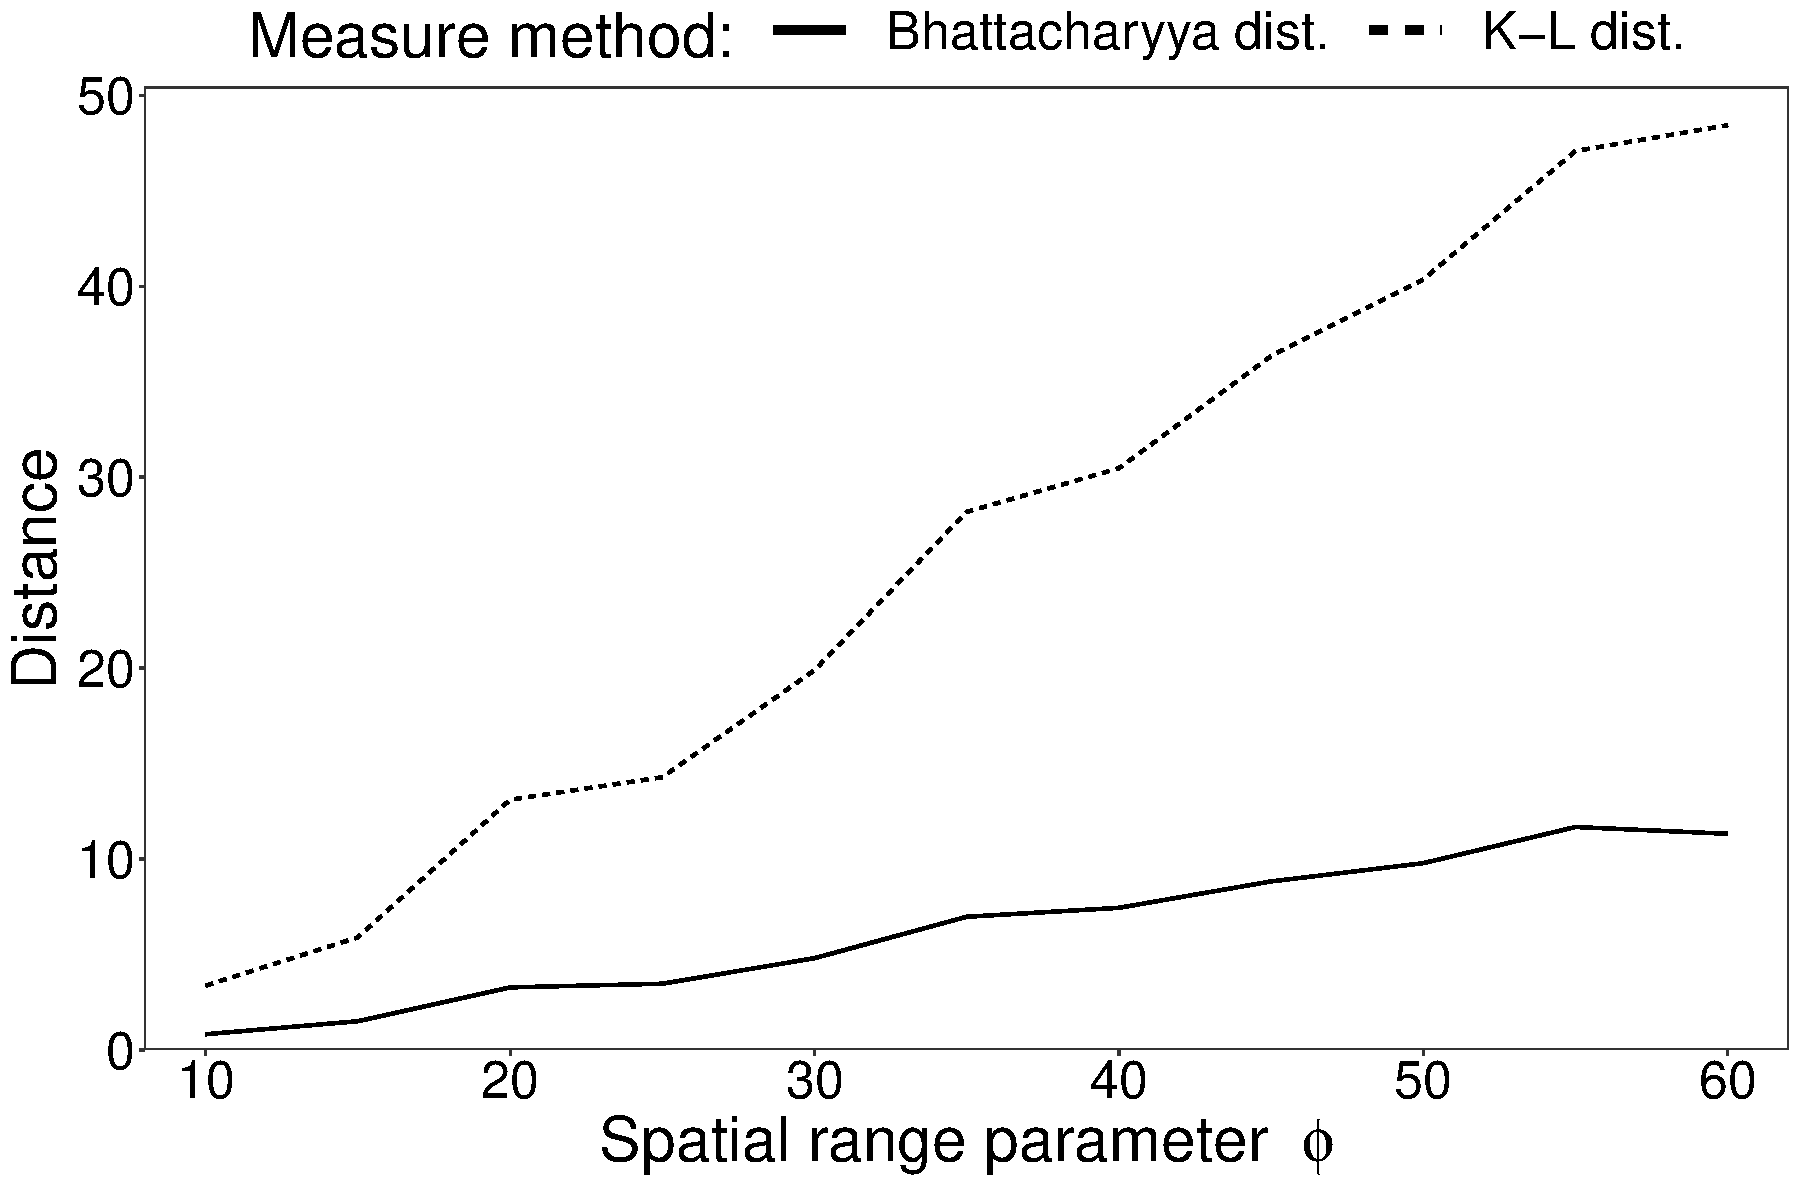
\includegraphics[width=8cm]{Figures/nnGP1.pdf} }
%{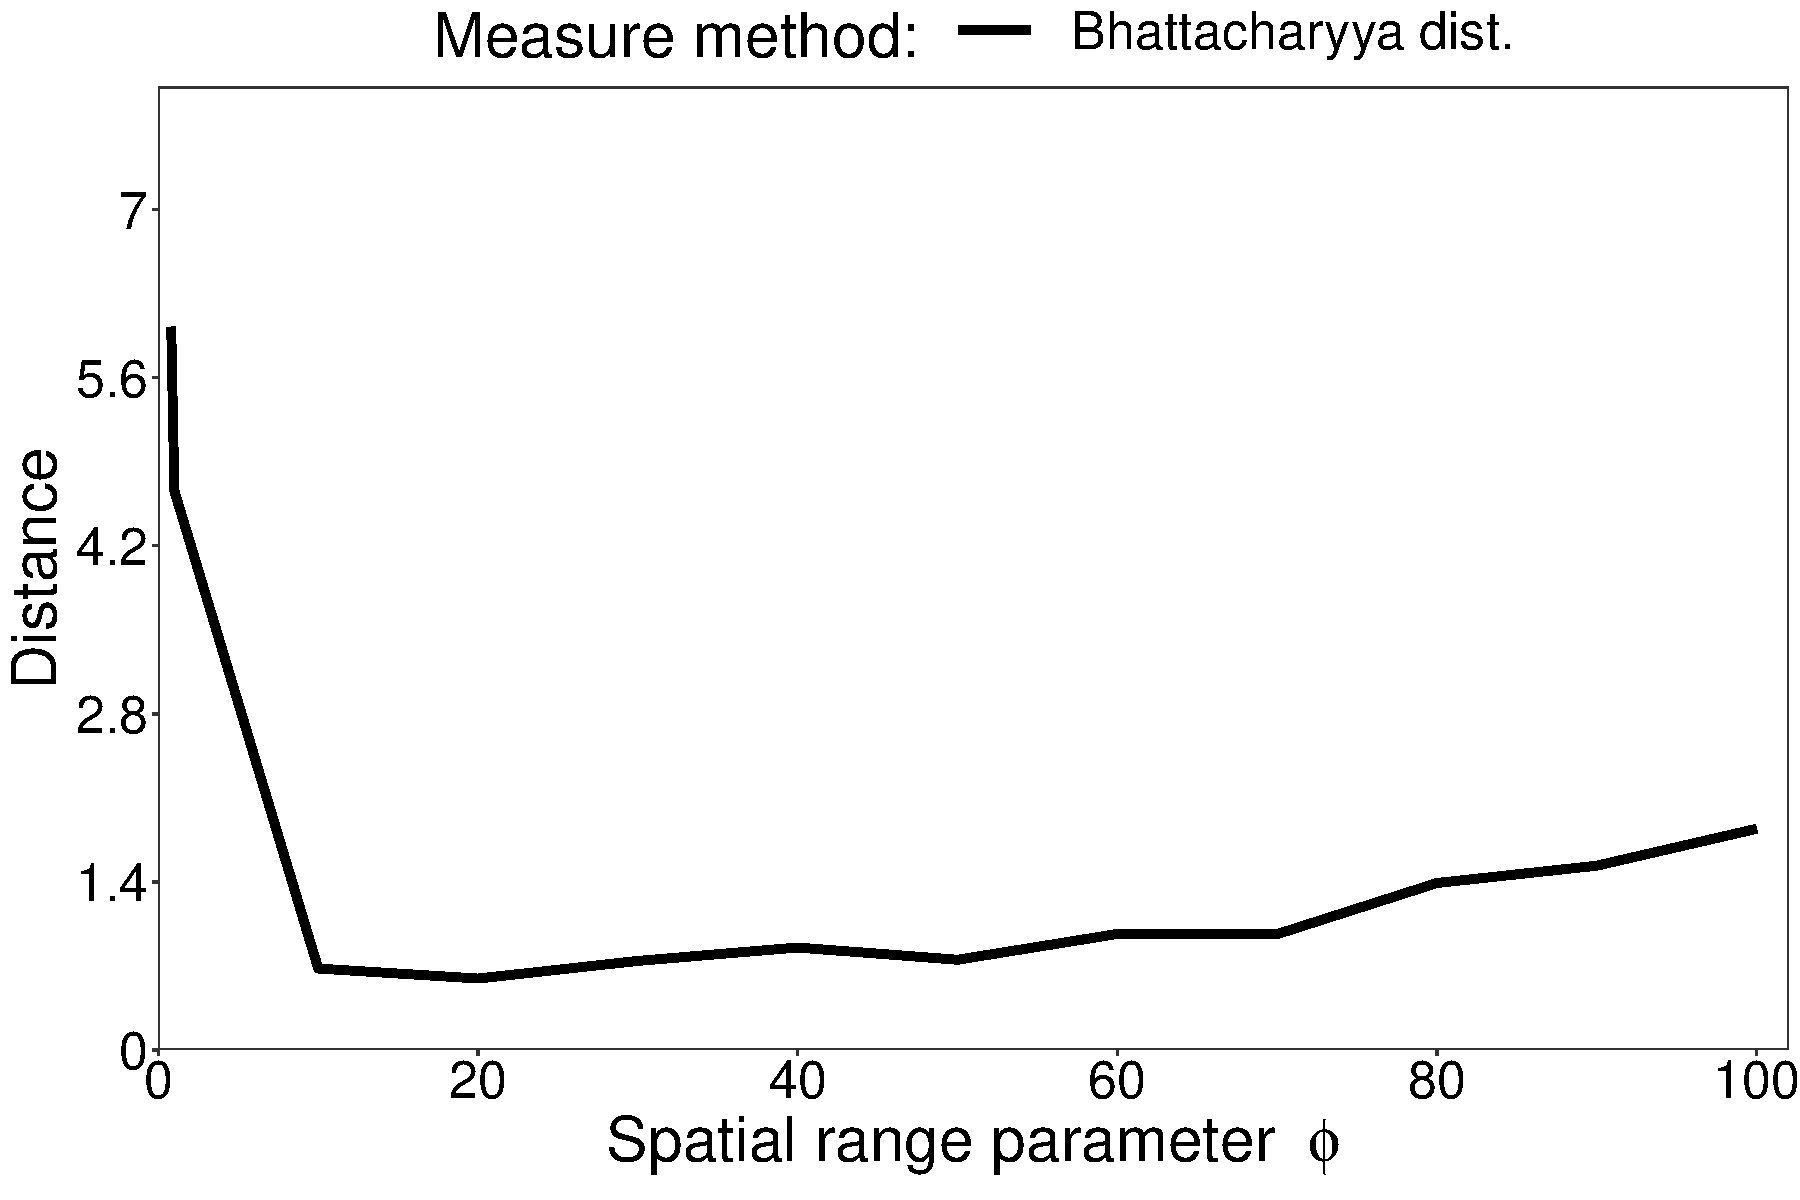
\includegraphics[width=8cm]{Figures/nnGP2.pdf} }
%{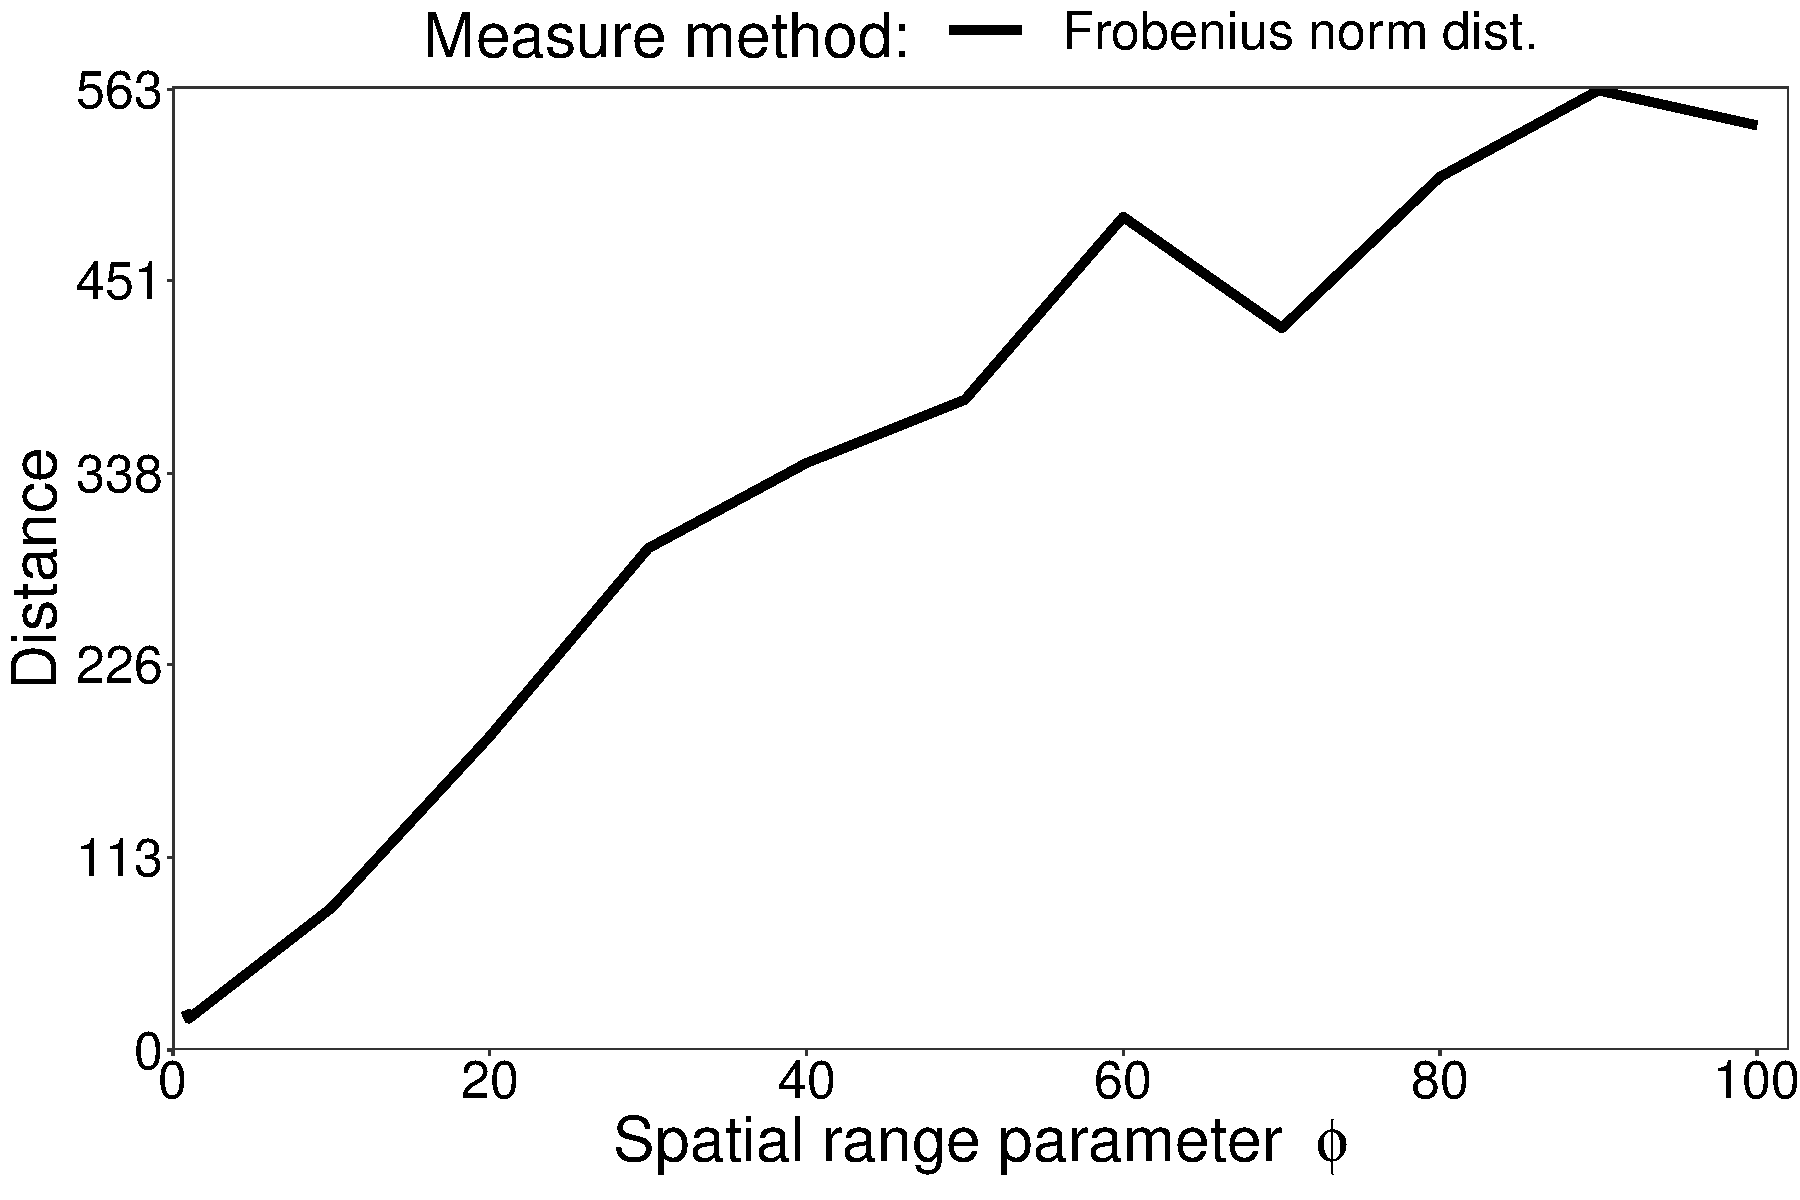
\includegraphics[width=8cm]{Figures/nnGP3.pdf} }
%\vspace{1em}
%\caption{The K-L distance, the Bhattacharyya distance and the Frobenius norm from the estimated covariance
%matrix to the true covariance matrix for the Matérn family with smoothness parameters $\nu = \frac{1}{2}$ and different spatial range parameters $\phi$. And this true covariance matrix at $500$ random locations from $[0, 100] \times [0, 100]$ was estimated by the NNGP model with $m = 20$  for 50 simulations.}\label{fig:nnGP1}
%\end{figure}
%
%\begin{figure}[H]
%{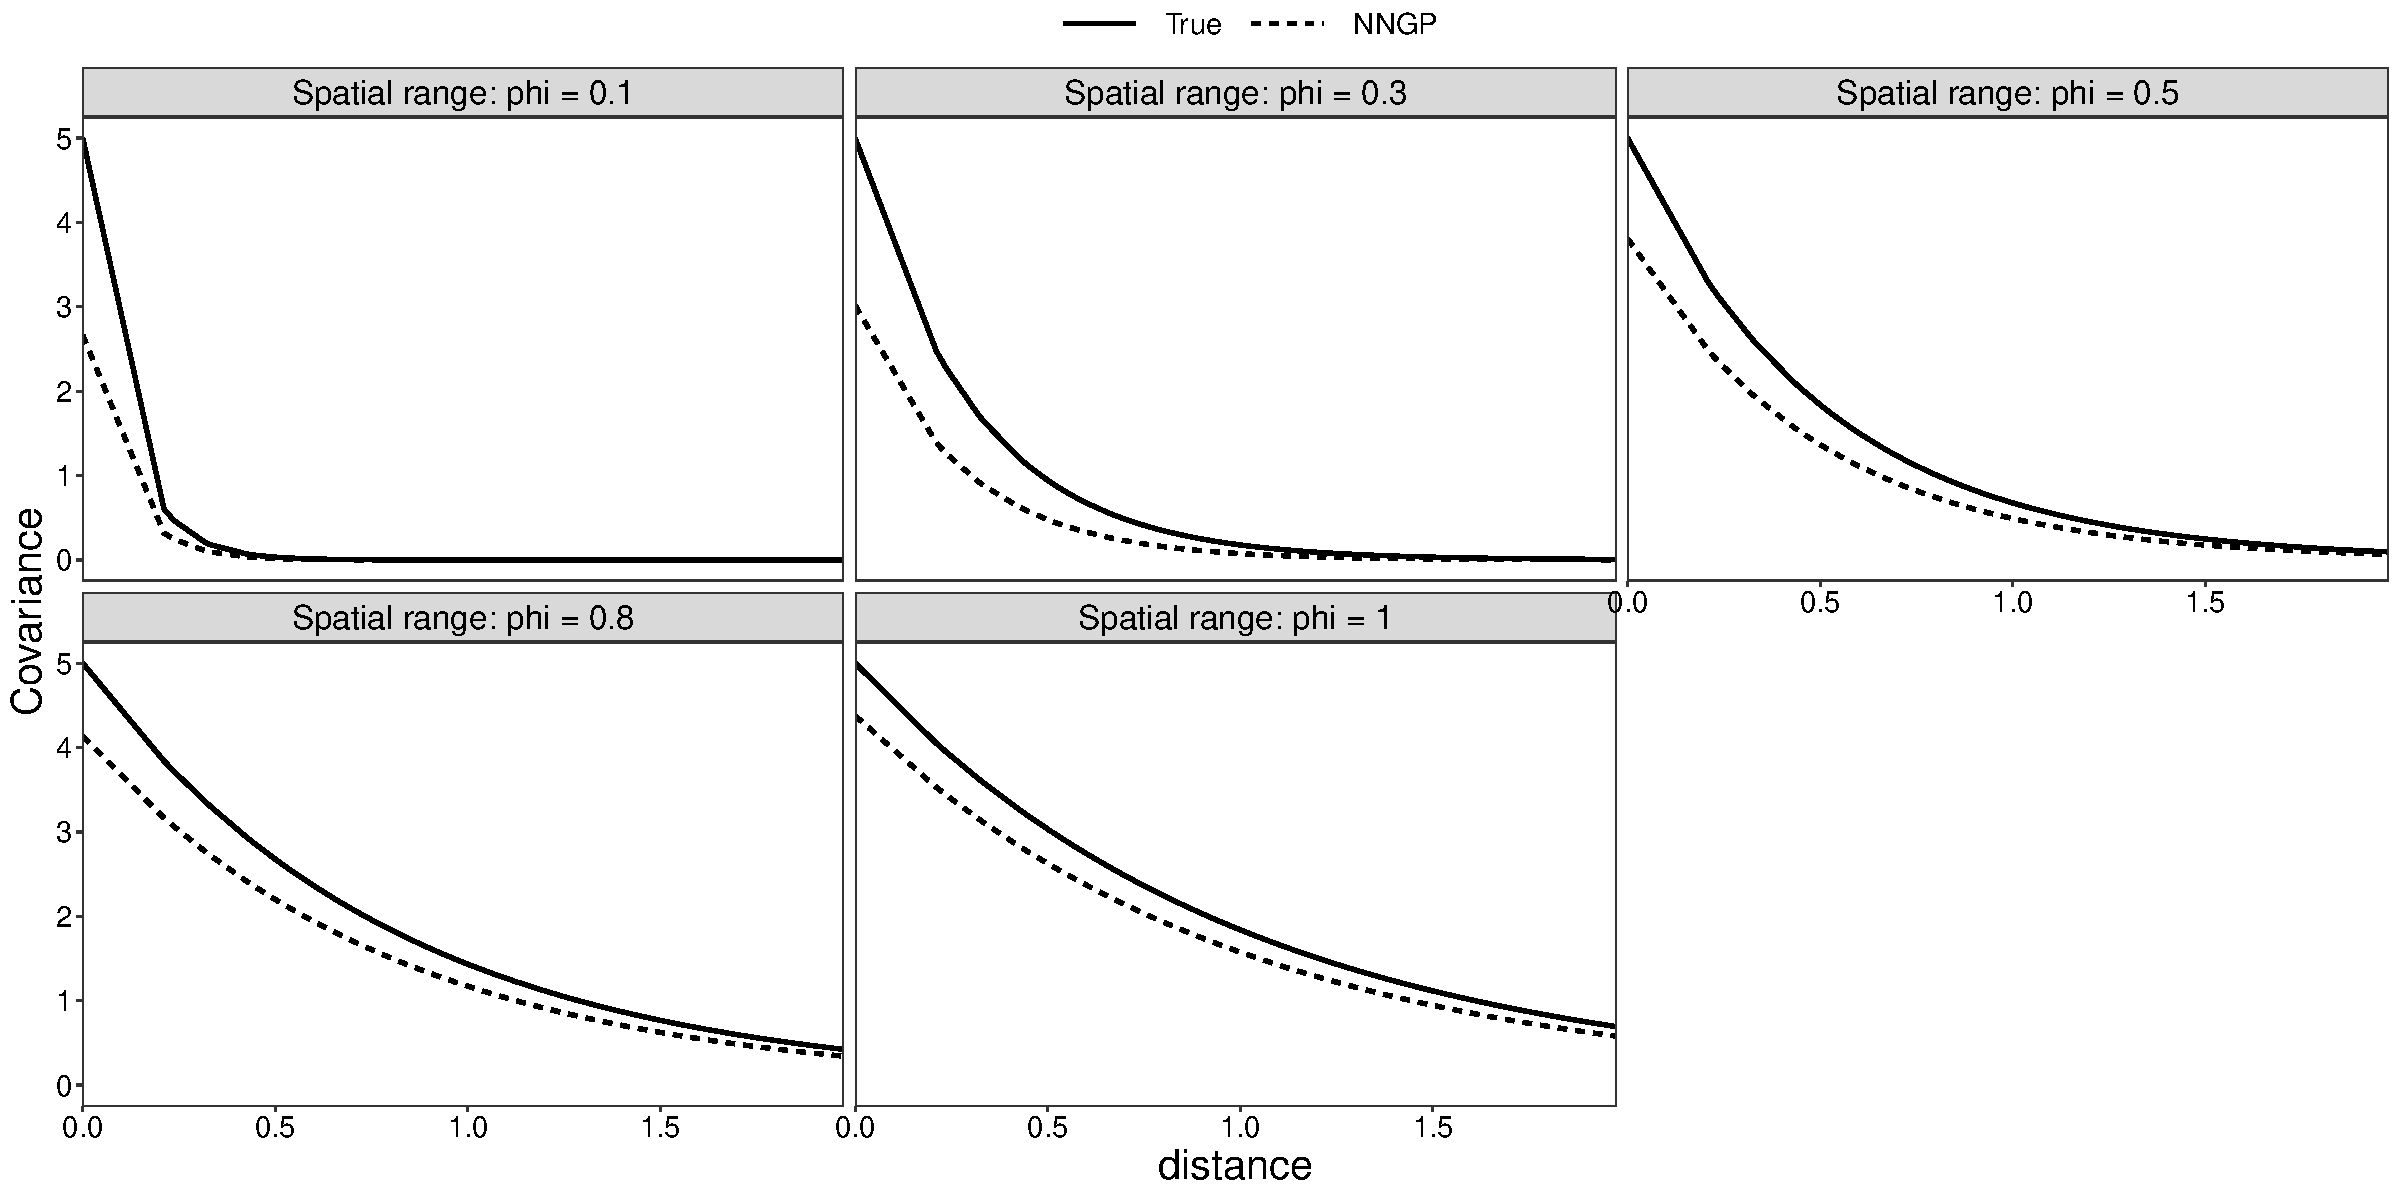
\includegraphics[width=18cm]{Figures/nnGP_Cov1.pdf} }
%{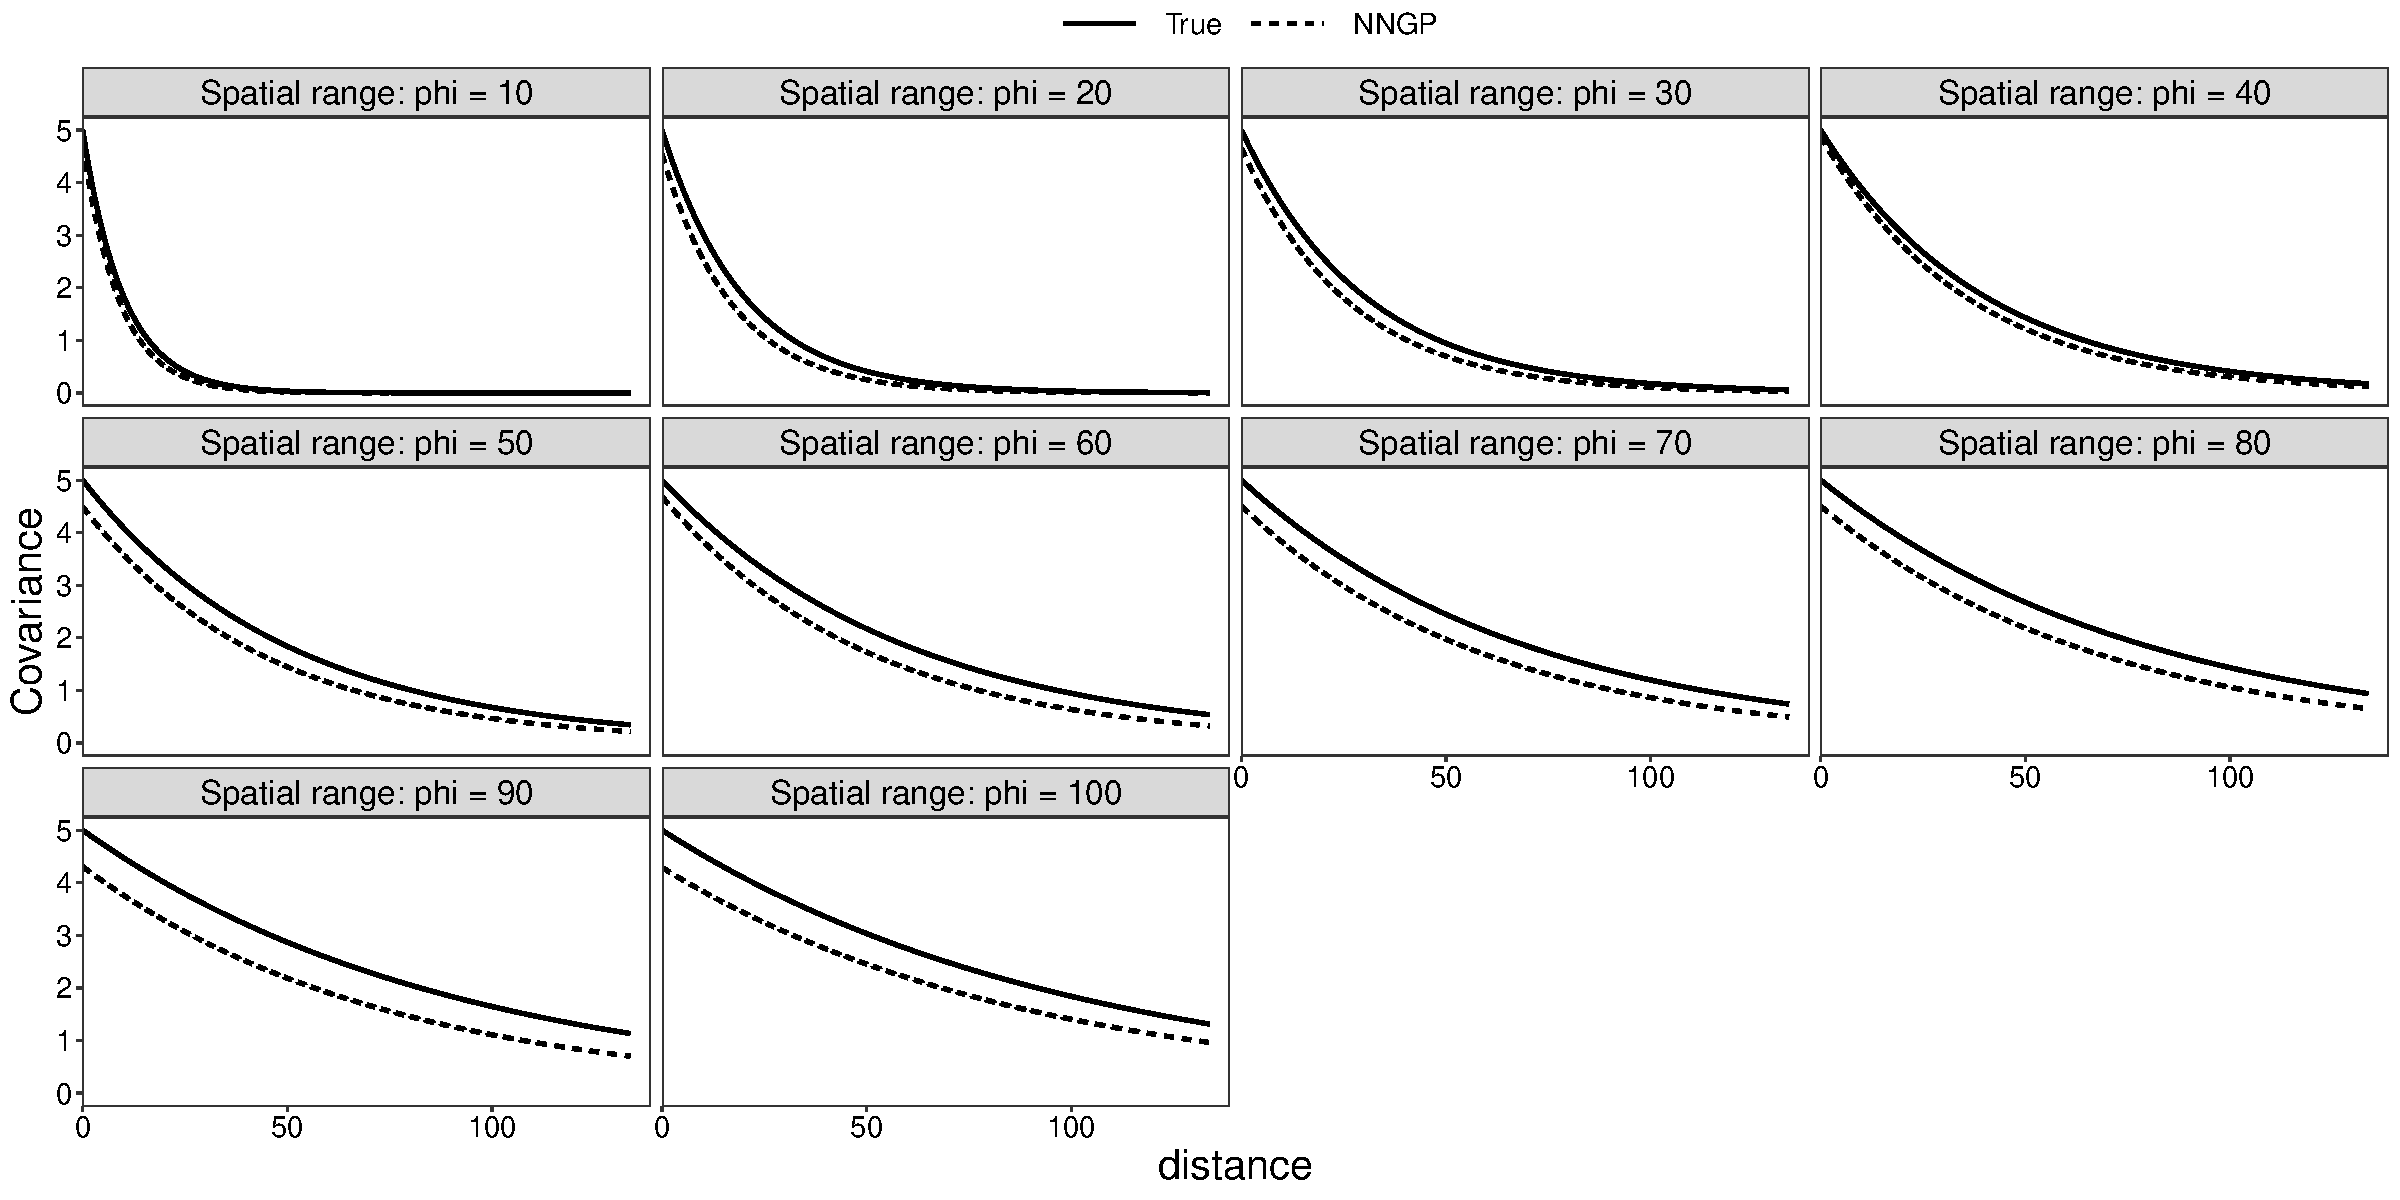
\includegraphics[width=18cm]{Figures/nnGP_Cov2.pdf} }
%\vspace{1em}
%\caption{Estimation results of covariance function corresponding to Figure \ref{fig:nnGP1}.}\label{fig:nnGP2}
%\end{figure}

%Figure \ref{fig:nnGP1} and \ref{fig:nnGP2} suggest that \textbf{the large-scale spatial dependencies for a larger domain can not be well-captured} by the NNGP, and at the same time, the top two panel of Figure \ref{fig:nnGP1} show that as with predictive process model, the NNGP may also \textbf{fail to capture some local information}, that may be related to the selection of reference set.
%Combing a NNGP $w(s)$ used to capture the \textcolor[rgb]{0.50,0.50,0.50}{local, small scale dependence structure} with its spatial smooth version $f(s)$ used to capture the \textcolor[rgb]{0.50,0.50,0.50}{large scale dependence structure}.

\section{\textcolor[rgb]{1.00,0.00,0.50}{Model specification}}
\begin{equation}
\begin{aligned}
  y(s) = \boldsymbol{x}(s)\boldsymbol{\beta} + w(s) + \epsilon(s).
\end{aligned} \label{model1}
\end{equation}
Let $\boldsymbol{w}(s) =  \sum_{l = 1}^{L}\sum_{k = 1}^{m_l}{h_k^{l}(s)\phi_k^l}$, where $\boldsymbol{h}^{l}$ is a pre-defined kernel function on the spatial $l$th grid-level  whose coefficients are denoted as $\boldsymbol{\phi}^l = \left(\phi_1^1, \cdots, \phi_{m_l}^l\right)$.

Specifically, we propose to estimate all parameters by minimizing the following objective function:
\begin{equation}\label{model2}
\frac{1}{n}\sum_{i = 1}^{n}\left\{y(s_i) -
\sum_{j = 1}^{p} \beta_jx_j(s_i) - \sum_{l = 1}^{L}\sum_{k = 1}^{m_l}{h_k^{l}(s_i)\phi_k}\right\}^2 +
%\sum_{j = 1}^{p}P_\lambda\left(\beta_j\right) +
\sum_{l = 1}^{L}\sum_{k = 1}^{m_l}P_\lambda\left(\phi_k^{l} - \sum_{j \in N(k)} v_j \phi_j^{l}\right)
\end{equation}
where $N(k)$ denotes the set of neighbors index of the vertice $k$.

\section{Some examples}
\subsection{Synthetic example from \href{https://chenyw68.github.io/Literature/[2018]A case study competition among methods for analyzing large spatial data.pdf}{\cite{heaton2019case}}}

The size of training data: 105, 569\\
The size of testing data: 44, 431\\
\begin{table}[H]
 \caption{RMSE for each competing method on the simulated data.}
  \centering
\begin{tabular}{rrrc}
\hlinewd{1pt}
    Method &    RMSE & Run time(min) \\
\hline
       FRK &      1.31  &            \\

   Gapfill &      1.00  &            \\

LatticKrig &      0.87  &            \\

      LAGP &      1.11  &            \\

Metakriging &      0.97  &            \\

       MRA &      0.83  &            \\

      NNGP &      0.88  &           70 \\

 Partition &      0.86  &            \\

Pre. Proc. &      1.43  &            \\

      SPDE &      0.86  &            \\

  Tapering &      0.97  &            \\

Periodic Embedding &    0.91  &            \\

\textbf{Model (\ref{model2})} &  0.86  &  35 \\
\hlinewd{0.8pt}
\end{tabular}
\end{table}

\subsection{Simulation study}
The \(n = 500\) spatial nonregularly points in
\([0, 50]\times [0, 50] \subset \mathcal{D}\) was randomly generated  by
\begin{equation} \label{fModel}
\boldsymbol{Y} =
\boldsymbol{W} + \boldsymbol{\varepsilon},
\end{equation}
where $\boldsymbol{\varepsilon}_t \sim N(\boldsymbol{0}, 0.5^2\boldsymbol{I})$ and $\boldsymbol{w} \sim GP\left(1 + \boldsymbol{X}_1\beta_1 + \boldsymbol{X}_2\beta_2, 15\exp\left(- \frac{\boldsymbol{D}}{10}\right) \right)$, the two covariates ($\boldsymbol{X}_1,  \boldsymbol{X}_2$) were, respectively, generated from $\texttt{beta}(20, 1)$ and $\texttt{beta}(2, 10)$ or $\texttt{N}(20, 1)$ and $\texttt{N}(2, 10)$ .

The 90\% of the samples were randomly selected as training set, the rest as test.  The testing results for model (\ref{model2}) and NNGP are as follows:
\begin{table}[H]
 \caption{Mean of RMSE and CRPS for the simulated data using 50 different seeds.}
  \centering
\begin{tabular}{rrrrc}
\hlinewd{1pt}
       nu  &      model &       RMSE &       CRPS  & Covariate $\boldsymbol{X}$ \\
\hline
      0.5  &       NNGP &      2.00  &      1.35  & \multirowcell{4}{beta dis.}\\

      0.5  &     Model (\ref{model2}) &      1.90  & 1.17 & \\

      2.0  &       NNGP &      1.02  &      0.89  & \\

      2.0  &     Model (\ref{model2}) &      0.86  &      0.74 & \\
 \hline
       2.0  &       NNGP &     1.23  &      11.87  &   \multirowcell{2}{Gaussian dis.}\\
       2.0  &     Model (\ref{model2}) &      0.99  &      11.86 & \\


\hlinewd{0.8pt}
\end{tabular}
\end{table}

  \begin{figure}[H]
    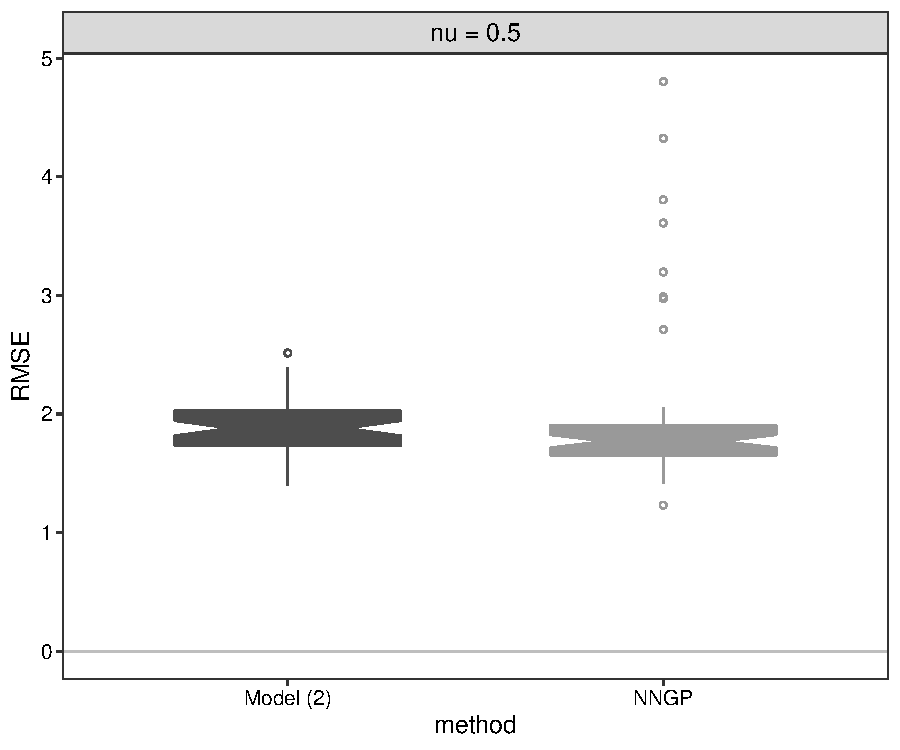
\includegraphics[width= 8cm]{./Figures/simuRMSE_1}
     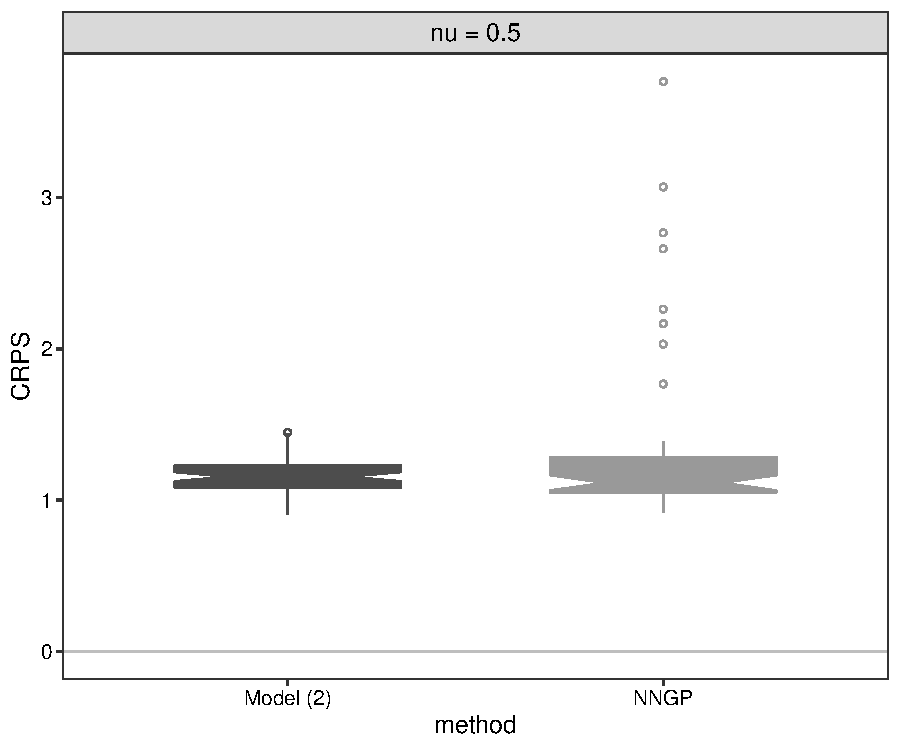
\includegraphics[width= 8cm]{./Figures/simuCRPS_1}\\
      \caption{Note that the covariance model(i.e. Matern function with the smoothness parameter $0.5$) is correctly specified for NNGP model. Left: RMSE for the two models. Right: CRPS for the two models.}
      \label{fgr:simulat1}
    \end{figure}

  \begin{figure}[H]
    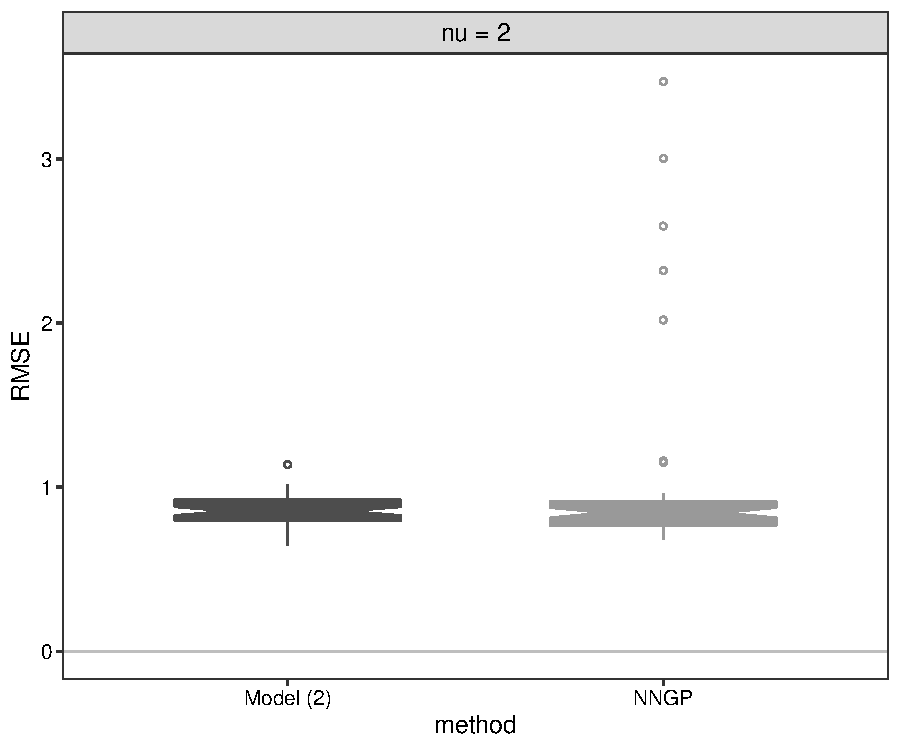
\includegraphics[width= 8cm]{./Figures/simuRMSE_2}
     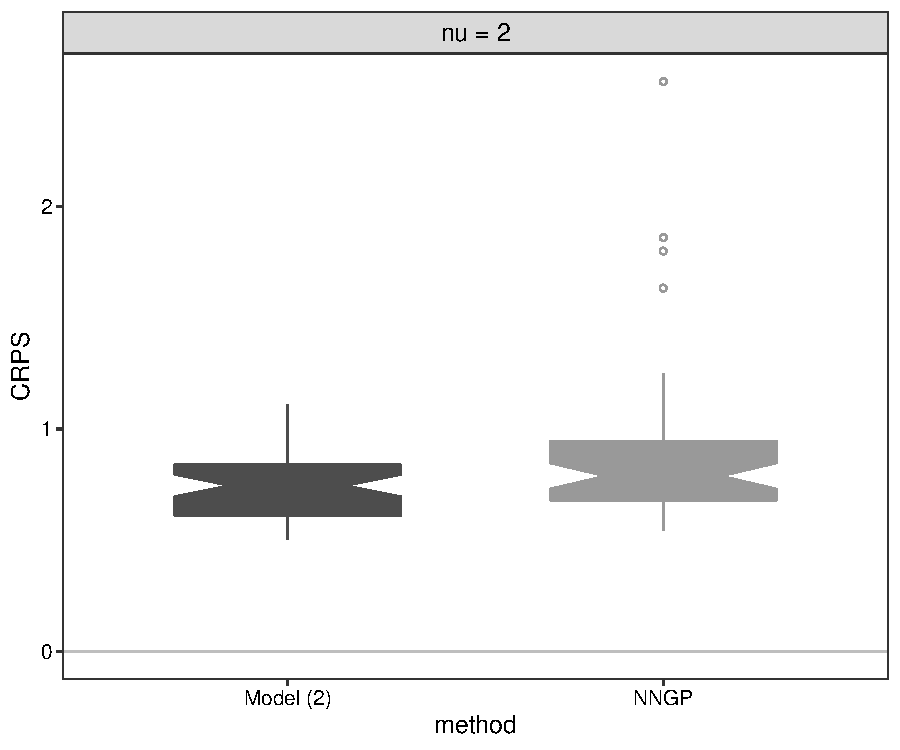
\includegraphics[width= 8cm]{./Figures/simuCRPS_2}\\
  \caption{Note that the NNGP covariance model is incorrectly specified and the specification is Matern function with the smoothness parameter $2$. Left: RMSE for the two models. Right: CRPS for the two models.}
      \label{fgr:simulat2}
    \end{figure}

      \begin{figure}[H]
    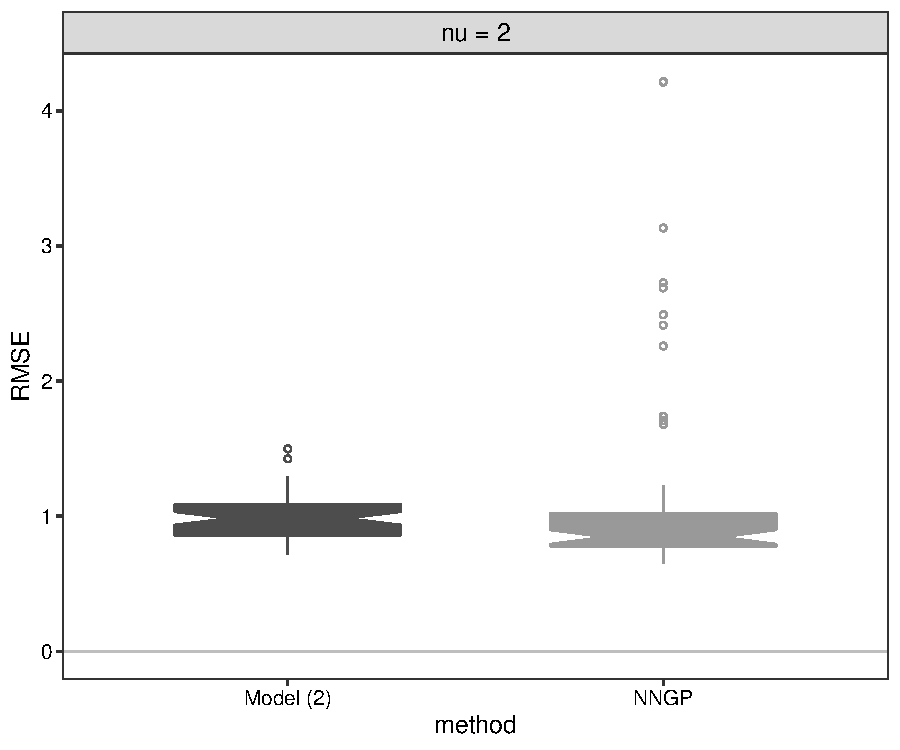
\includegraphics[width= 8cm]{./Figures/simuRMSE_3}
     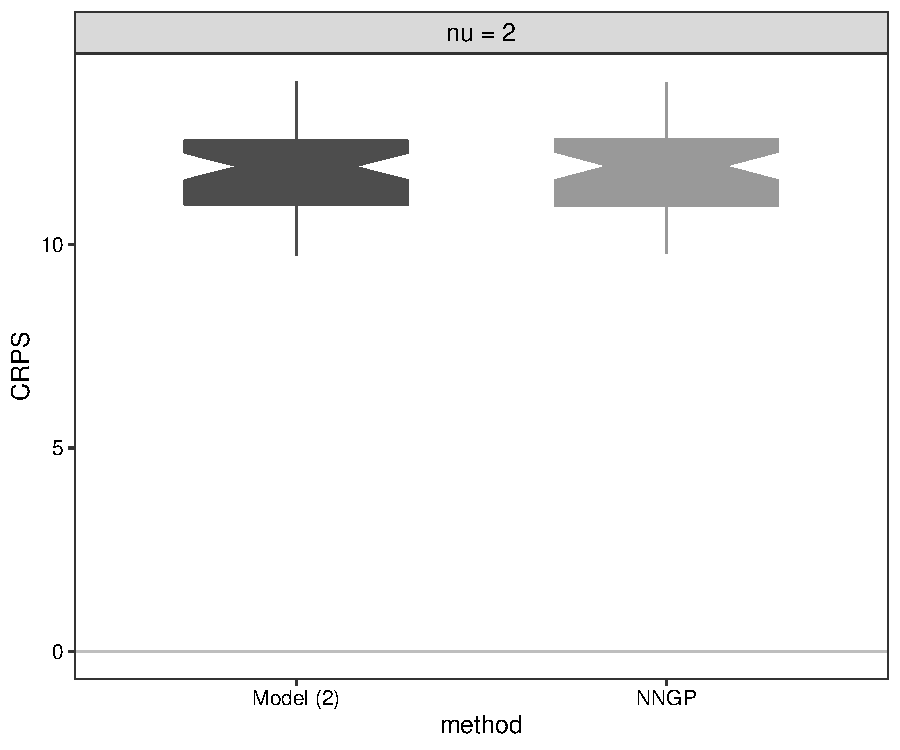
\includegraphics[width= 8cm]{./Figures/simuCRPS_3}\\
  \caption{The covariate $\boldsymbol{X}$ are from Gaussian distribution.}
      \label{fgr:simulat2}
    \end{figure}

\subsection{Real data from Beijing-Tianjin-Hebei region}
  \begin{figure}[H]
    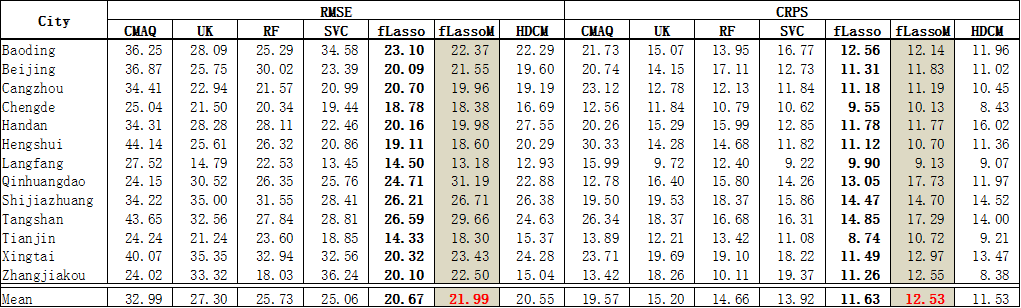
\includegraphics[width= 16cm]{./Figures/fuse_lasso_s}\\
    (a)\\
     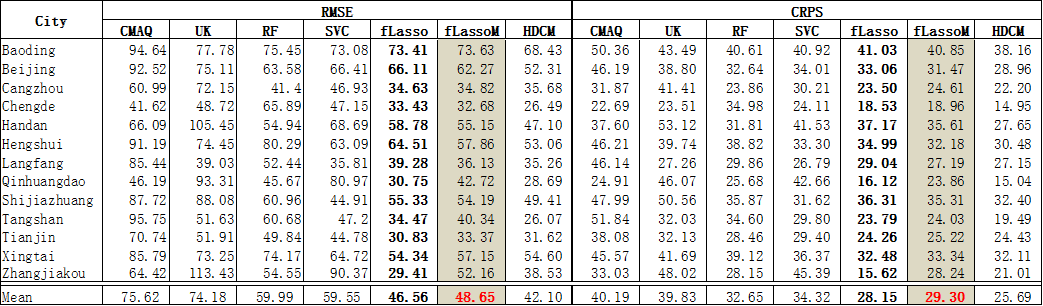
\includegraphics[width= 16cm]{./Figures/fuse_lasso_w}\\
     (b)\\
      \caption{(a):The cross validation for the warm season with the $6$ different models. (b): The cross validation for the cool season with the $6$ different model. The label ``\texttt{fLasso}''  corresponds to model (\ref{model2}) and the label ``\texttt{fLassoM}'' is a multi-variable version.}
      \label{fgr:cmaq_obs}
    \end{figure}
%----------------------------------------------------------------------------------------
%\bibliographystyle{achemso}
\bibliography{summary_spatial}
\end{document} 